\section{Parsing models performance}

The performance of the models trained here is lower than of those used by default by the parsers. This can be explained by the training parameters, specifically by the batch size, which was set to a 1000 for every training. A smaller batch size could possibly improve the performance, but this could not be tested here due to limited resources.

The combined model trained on UD data perfomed significantly better than the model trained on SUD according to both measures calculated here. This is contrary to what was expected based on the previous studies on learnability of dependency schemes. One possible explanation for this outcome is that SUD-trained models do not perform well when trained on mixed domain data. Despite the poor performance of the combined SUD model, the spoken SUD model performed better (according to the LAS score) than the UD-trained one. Additionally, in the study conducted by \cite{tuo:prz:lac:21} the model for parsing English was trained only on the English Web Treebank. Both of the data sources for those models are more homogenous than the data for the combined model trained for this study, which included for instance academic texts, travel guides, public talk transcripts and emails. 

Two additional models were trained to see if constricting the training data to written sources boosts the performance of the SUD-trained model compared to the UD-trained one. Training data chosen for this purpose was the same as for the combined model, but without the parts of the GUM corpus chosen for the spoken model (documents tagged as vlogs, interviews and conversations). The results of the automatic evaluation conducted on those models are presented in Table \ref{tab:written}. 

\begin{table}
\centering
\begin{tblr}{
    cells = {c},
	cell{1}{1} = {c=6}{c},
	cell{2}{1,4} = {c=3}{c},
    hlines, vlines}
    written model & & & & & \\
    UAS & & & LAS & & \\
    UD & SUD & $\Delta$ & UD & SUD & $\Delta$ \\
    89.98 & 89.03 & \textbf{0.95} & 87.58 & 86.89 & \textbf{0.69}
\end{tblr}
\caption{\centering UAS and LAS for the models trained on UD and SUD corpora containg only texts from written sources. Significant differences between the scores are in bold.}\label{tab:written}
\end{table}

The UD-trained model achieved significantly better performance, both when measured in UAS and LAS. It is possible that the training data for those models were still too diverse compared to the spoken model -- sources ranged from online reviews to legal texts. To find if any of the annotation schemes is better for parsing diverse or more specific data, further research should be conducted.

\section{Manual evaluation results}

The manual evaluation showed that the SUD-based extraction of coordinations was more accurate, but not significantly. One reason for weaker performance of the SUD-based approach than expected could be the reliance on the \texttt{Shared} feature. As was presented in Section \ref{sec:shared-deps}, some dependencies in SUD trees are marked as shared by the whole coordination by adding a \texttt{Shared=Yes} feature to their morphological features. To also add this information to the parsed trees for the COCA corpus, a part-of-speech tagger from the Stanza pipeline was trained additionally to the dependency parser. The number of words with this feature in the training datasets could be too small for the model to properly learn when this feature should be added. In the manual evaluation, 13.6\% of the coordinations extracted incorrectly using the SUD-based approach would be extracted correctly if the \texttt{Shared} feature was not given priority when deciding which dependents are part of the conjunct. It is however unclear how many of the coordinations would not have been extracted correctly without that feature, therefore this issue requires further investigation. 

The evaluation itself has some limitations. A bigger and better balanced sample size should be evaluated -- here the evaluated coordinations were those found in the testing sets of the corpora used for training. The coordinations found there did not have sufficient representation of coordinations of different length differences and different governor positions. While this evaluation gives some insight into the accuracy of the approaches, a more thorough evaluation should be conducted to investigate the cons of each approach.

\section{Compatibility of corpus data and different approaches to coordination}\label{sec:which-approach}

% \begin{wrapfigure}{L}{0.4\textwidth}
% \adjincludegraphics[scale=.5, trim={0 0 {.5\width} 0}, clip]{inputs/sud-modelled.pdf}\caption{Modelled proportions of coordinations with shorter left conjunct depending on the length difference between the conjuncts, data according to
% the SUD-trained model with lengths measured in words (subfigure of Figure \ref{fig:sud-logit}).}\label{idk-figure}
% \end{wrapfigure}

Figure \ref{idk-figure} shows how the proportion of coordinations with shorter left conjuncts changes with the length difference between the leftmost and rightmost conjuncts and depending on the position of the governor. Corpus data presented in the figure is immediately incompatible with the asymmetrical approaches, according to which the tendency to put shorter conjuncts on the left should always increase, regardless of the gorvernor position. The Prague or conjunction-headed approach is not compatible either, because with the governor on the right the tendency for the shorter conjunct to appear on the left decreases significantly, when according to this approach it should be stable. 

\begin{figure}[H]
    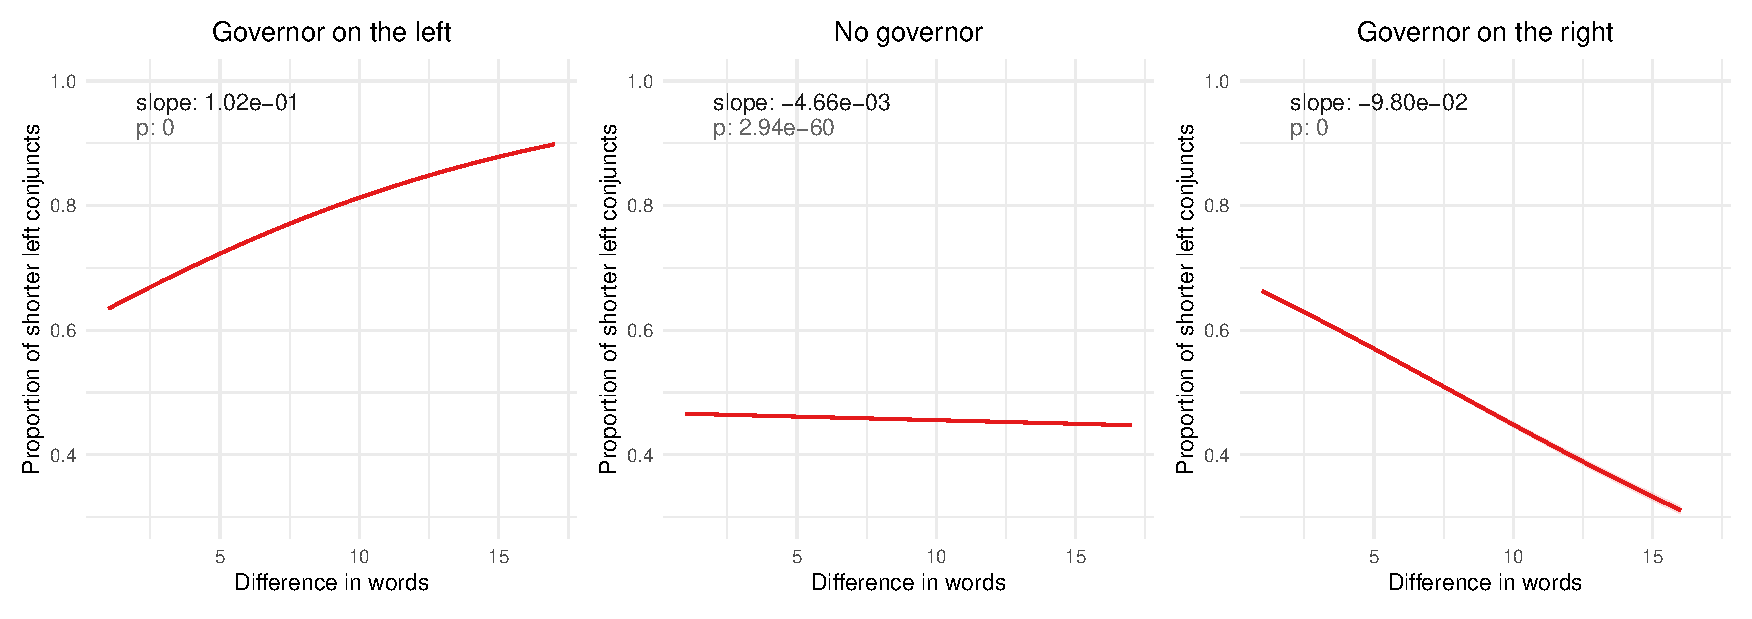
\includegraphics[width=\textwidth]{inputs/halfofsudmodelled.pdf}
    \caption{Modelled proportions of coordinations with shorter left conjunct depending on the length difference between the conjuncts, data according to the SUD-trained model with lengths measured in words (subfigure of Figure \ref{fig:sud-logit}).}\label{idk-figure}
\end{figure}

Among the four approaches described here, the one supported the most by corpus data is the London or multi-headed approach. Diagrams (\ref{ex:london-all}) from Section \ref{sec:london} presenting this annotation style are repeated here as (\ref{ex:london-again}). (\ref{ex:london-again}a--b) demonstrate that when the governor is on the left, the depenencies are minimised when the shorter conjunct is also on the left. This is compatible with the top plot in Figure \ref{idk-figure}, where the bigger the difference between conjunct lenghts (and therefore the bigger the pressure of the DLM effect for ordering conjuncts in a way that minimises dependency lengths), the more coordinations have their shorter conjunct on the left. Similarly when the governor is on the right -- (\ref{ex:london-again}e--f) show that the shorter conjunct should also be placed on the right to minimise the dependency lengths and the bottom plot in Figure \ref{idk-figure} confirms that there is a tendency to do that. 

The issue becomes more complex when looking at the middle plot in Figure \ref{idk-figure}. The slope is significantly negative, therefore the chance of no tendency being present is very low, which is not compatible with the predictions of the London approach. According to (\ref{ex:london-again}c--d) there should be no tendency in any direction, as neither of the conjunct placements minimises the dependency lengths. 

\begin{exe}
\ex\label{ex:london-again}
\begin{minipage}[t]{2.5\treewidth}
\begin{xlist}

\begin{multicols}{2}

\ex
\begin{minipage}[b][\treeheight]{\treewidth}
\vfill
% gov on the left, shorter conj on the left
\begin{dependency}[theme = simple, baseline=-\the\dimexpr\fontdimen22\textfont2\relax]
    \begin{deptext}
        $\odot$\&$\diamond$\&$\diamond$\&$\square$\&$\diamond$\&$\diamond$\&$\diamond$\&$\diamond$\&$\diamond$\\
    \end{deptext}
    \depedge{1}{2}{}
    \depedge{1}{5}{}
    \depedge{5}{4}{}
    \wordgroup{1}{2}{3}{}
    \wordgroup{1}{5}{9}{}
\end{dependency}
\end{minipage}

\columnbreak

\ex
\begin{minipage}[b][\treeheight]{\treewidth}
% gov on the left, shorter conj on the right
\begin{dependency}[theme = simple, baseline=-\the\dimexpr\fontdimen22\textfont2\relax]
    \begin{deptext}
        $\odot$\&$\diamond$\&$\diamond$\&$\diamond$\&$\diamond$\&$\diamond$\&$\square$\&$\diamond$\&$\diamond$\\
    \end{deptext}
    \depedge{1}{2}{}
    \depedge{1}{8}{}
    \depedge{8}{7}{}
    \wordgroup{1}{2}{6}{}
    \wordgroup{1}{8}{9}{}
\end{dependency}
\end{minipage}
\end{multicols}

\begin{multicols}{2}

\ex
\begin{minipage}[b][\treeheight]{\treewidth}
\vfill
% gov absent, shorter conj on the left
\phantom{$\odot$}\hspace{\fontdimen4\font}
\begin{dependency}[theme = simple, baseline=-\the\dimexpr\fontdimen22\textfont2\relax]
    \begin{deptext}
        $\diamond$\&$\diamond$\&$\square$\&$\diamond$\&$\diamond$\&$\diamond$\&$\diamond$\&$\diamond$\\
    \end{deptext}
    \deproot[edge height=4ex]{1}{}
    \deproot[edge height=4ex]{4}{}
    \depedge{4}{3}{}
    \wordgroup{1}{1}{2}{}
    \wordgroup{1}{4}{8}{}
\end{dependency}
\end{minipage}

\columnbreak

\ex
\begin{minipage}[b][\treeheight]{\treewidth}
% gov absent, shorter conj on the right
\phantom{$\odot$}\hspace{\fontdimen4\font}
\begin{dependency}[theme = simple, baseline=-\the\dimexpr\fontdimen22\textfont2\relax]
    \begin{deptext}
        $\diamond$\&$\diamond$\&$\diamond$\&$\diamond$\&$\diamond$\&$\square$\&$\diamond$\&$\diamond$\\
    \end{deptext}
    \deproot[edge height=4ex]{1}{}
    \deproot[edge height=4ex]{7}{}
    \depedge{7}{6}{}
    \wordgroup{1}{1}{5}{}
    \wordgroup{1}{7}{8}{}
\end{dependency}
\end{minipage}
\end{multicols}

\begin{multicols}{2}

\ex
\begin{minipage}[b][\treeheight]{\treewidth}
% gov on the right, shorter conj on the left
\phantom{$\odot$}\hspace{\fontdimen4\font}
\begin{dependency}[theme = simple, baseline=-\the\dimexpr\fontdimen22\textfont2\relax]
    \begin{deptext}
        $\diamond$\&$\diamond$\&$\square$\&$\diamond$\&$\diamond$\&$\diamond$\&$\diamond$\&$\diamond$\&$\odot$\\
    \end{deptext}
    \depedge{9}{1}{}
    \depedge{9}{4}{}
    \depedge{4}{3}{}
    \wordgroup{1}{1}{2}{}
    \wordgroup{1}{4}{8}{}
\end{dependency}
\end{minipage}

\columnbreak

\ex
\begin{minipage}[b][\treeheight]{\treewidth}
% gov on the right, shorter conj on the right
\phantom{$\odot$}\hspace{\fontdimen4\font}
\begin{dependency}[theme = simple, baseline=-\the\dimexpr\fontdimen22\textfont2\relax]
    \begin{deptext}
        $\diamond$\&$\diamond$\&$\diamond$\&$\diamond$\&$\diamond$\&$\square$\&$\diamond$\&$\diamond$\&$\odot$\\
    \end{deptext}
    \depedge{9}{1}{}
    \depedge{9}{7}{}
    \depedge{7}{6}{}
    \wordgroup{1}{1}{5}{}
    \wordgroup{1}{7}{8}{}
\end{dependency}
\end{minipage}
\end{multicols}

\end{xlist}
\end{minipage}
\end{exe}
\vspace{6ex}

A look at the plots in the Appendix \ref{ap:genres}, which shows the tendencies in conjunct placement in different styles, could explain why the middle plot in Figure \ref{idk-figure} looks differently than expected. In most of the plots, the fluctuations in proportions of shorter left conjuncts when the coordination has no governor are small. The only plots that stand out in this matter are the ones for spoken data and data from TV and movies. According to \cite{davies-tvm}, the data in the TV and movies section of the COCA corpus is a good representation of the spoken, informal English, because the source of this data are mostly subtitles from TV shows and movies. It has also been shown that spoken English has a smaller tendency towards minimising dependency lengths than written English \citep{liu-2019-comparative}. If the spoken English language (represented here by the spoken and TV/movies subsets of COCA) does not minimise dependency lengths, then the results from this data cannot point to any of the annotation schemes based on the DLM effect. Appendix \ref{ap:written} shows the modelled plots after excluding the spoken and TV/movies data -- the slopes are less negative and the p-value is larger. 

The annotation scheme most compatible with the results shown in Figure \ref{idk-figure} is therefore the London approach. This is not however fully compatible with the results from the spoken data, which should be studied with more detail in the future. An important point here is that the study was conducted solely on the English language. Conducting similar studies on different languages could give a better insight into how coordinations are interpreted. 

\section{Difference between the data resulting from different annotation schemes}

% they needed the grammaticalisation, i dont have any grammaticalisation here. there are differences between sud and ud data and i think the reason their data was skewed was that they used ud, which did in fact influence the results

Figures \ref{fig:sud-observed} and \ref{fig:ud-observed} show the proportions of coordinations with shorter left conjuncts extracted from the same corpus, but the plots look different. The difference between the data used for those plots is the approach in which the coordinations were analised -- Figure \ref{fig:sud-observed} shows the data from the SUD-based approach and Figure \ref{fig:ud-observed} from the UD-based approach. 

Plots from Figure \ref{fig:ud-observed} resemble those from \cite{prz:etal:24}, because the same corpus and the same (UD-based) approach was used there.\footnote{There are some differences between those plots and three main factors can explain them: 1) the parsing model used here may be less accurate and therefore some of the coordinations could be extracted differently, 2) the spoken parts of the COCA corpus were included in the current study, but not in the previous one and 3) the current study is based on the whole COCA corpus, whereas the previous study used only parts of the corpus. As for the difference in model performance between the UD-trained model here and the default Stanza model for English used by \cite{prz:etal:24}, it is not possible to say which model is more accurate, because the accuracy scores of the combined Stanza model for English were not published.} Authors of the provious study suspected that the DLM effect in coordinations was grammaticalised and because of that all of the tendencies in the plots were more positive, than if the DLM effect was working only at the level of usage. If that were the case, then the grammaticalisation would be also visible in the data from the SUD-based approach. Since that is not the case, it can be argued that it was the UD annotation scheme that influenced the results.
%ARTYKUL SANTIAGO MOZE MA TU SENS???
Specifically, the difference between annotation schemes that can explain the differences observed here is the one that was mentioned in Section \ref{sec:sud criteria}. Because of the choice to have the content words as dependency heads, in some coordinations finding the extent of the left conjunct is impossible. In the troubling example (\ref{ex:UD magma}) (repeated here as (\ref{ex:rep-UD-magma})), the left conjunt is cut according to the UD-based approach. If this mistake happens often enough in the corpus, it could cause the proportion of coordinations with shorter left conjuncts to be bigger than it actually is. In the plots the difference appears mainly in coordinations with smaller length differences between the conjuncts and the coordination in (\ref{ex:rep-UD-magma}) is an example of those. Making sure that this is the cause for differences in results requires further investigation. 

\begin{figure}
\begin{exe}
	\ex\label{ex:rep-UD-magma}
	\begin{dependency}[hide label, baseline=-\the\dimexpr\fontdimen22\textfont2\relax]
		\begin{deptext}
			This\& magma\& often\& does\& not\& reach\& the\& surface\& but\& cools\& at\& depth.\\
		\end{deptext}
	\depedge{2}{1}{det} 
	\depedge[show label]{6}{2}{nsubj} 
	\depedge[show label]{6}{3}{advmod} 
	\depedge[show label]{6}{4}{aux} 
	\depedge[show label]{6}{5}{advmod} 
	\deproot[show label, edge height=3cm]{6}{root} 
	\depedge{8}{7}{det} 
	\depedge{6}{8}{obj} 
	\depedge[show label]{10}{9}{cc} 
	\depedge[show label, edge height=2cm, theme=night]{6}{10}{conj} 
	\depedge{12}{11}{case} 
	\depedge[show label]{10}{12}{obl} 
	
	\depedge[edge below]{2}{1}{det} 
	\depedge[edge below, show label]{4}{2}{subj} 
	\depedge[edge below, show label]{4}{3}{mod} 
	\deproot[edge below, show label, edge height=2cm]{4}{root} 
	\depedge[edge below]{4}{5}{mod} 
	\depedge[edge below]{4}{6}{comp:aux} 
	\depedge[edge below]{8}{7}{det} 
	\depedge[edge below]{6}{8}{comp:obj} 
	\depedge[edge below, show label]{10}{9}{cc} 
	\depedge[edge below, show label, edge height=1.5cm, theme=night]{4}{10}{conj}
	\depedge[edge below, show label]{10}{11}{udep} 
	\depedge[edge below]{11}{12}{comp:obj}
\end{dependency}
\end{exe}
\caption{Sentence \texttt{w01031015} from the PUD corpus \citep{pud} with a UD dependency tree above the text and a SUD dependency tree below the text.}
\end{figure}	

It is also worth noting that the same coordination can have different governor positions in each annotation scheme. This is illustrated with a UD tree in (\ref{ex:ud-heads}) and a corresponding SUD tree in (\ref{ex:sud-heads}), where the coordination \textsl{efficient and accurate} does not have a governor according to UD, but has a governor on the left according to SUD. It requires further research how many of the coordinations in the whole dataset have ambiguous governor positions like this. Of the coordinations in the manual evaluation, 15\% had different governor positions depending the annotation scheme, which could affect the results of the analysis presented in Section \ref{sec:which-approach}.

\begin{figure}[H]
\begin{exe}
\ex\label{ex:ud-heads}
\begin{dependency}[baseline=-\the\dimexpr\fontdimen22\textfont2\relax]
	\begin{deptext}[column sep=.4cm]
			This\& system\& is\& efficient\& and\& accurate.\\
		\end{deptext} 
	\depedge{2}{1}{det} 
	\depedge{4}{2}{nsubj} 
	\depedge{4}{3}{cop} 
	\deproot[theme=night]{4}{root} 
	\depedge{6}{5}{cc} 
	\depedge{4}{6}{conj} 
\end{dependency}
\end{exe}

\begin{exe}
\ex\label{ex:sud-heads}
\begin{dependency}[baseline=-\the\dimexpr\fontdimen22\textfont2\relax]
	\begin{deptext}[column sep=.4cm]
			This\& system\& is\& efficient\& and\& accurate.\\
		\end{deptext} 
	\depedge{2}{1}{det} 
	\depedge{3}{2}{subj} 
	\deproot{3}{root} 
	\depedge[theme=night]{3}{4}{comp:pred} 
	\depedge{6}{5}{cc} 
	\depedge{4}{6}{conj} 
\end{dependency}
\end{exe}
\caption{Fragment of the sentence \texttt{GUM\_academic\_census-25} with a UD tree in (\ref{ex:ud-heads}) and a SUD tree in (\ref{ex:sud-heads}). The governor of the coordination is marked with a dark label -- in the UD tree that label is \texttt{root}, therefore the coordination does not have a governor.}
\end{figure}

This difference cannot explain why the results from the UD-based and SUD-based approach were different, but it should be mentioned because it affects one of the main explanatory variables used in the analysis of coordinations presented here and in \cite{prz:etal:24}. One way to avoid this issue is to analyse constituency trees instead of dependency trees, as was done by \cite{prz:woz:23}. The information about the governor position was not explicitly available in their treebank, but the rules they applied for finding the position of the governor were evaluated to be 97\% accurate. This way the data is not skewed by any decisions made by the annotation scheme creators. 

%moze trzeba to robic tylko na skladnikowych? moze mozna na zaleznosciowych ale tylko sud? czy mam za tym argumenty?
